\documentclass[12pt]{article}

\usepackage[margin=1in]{geometry} % 1-inch margins
\usepackage{times}                % Times New Roman font
\usepackage{fancyhdr}             % Custom header/footer
\usepackage{titlesec}             % Custom section formatting
\usepackage{setspace}             % Line spacing
\usepackage{indentfirst}      
\usepackage{graphicx}

% Indent first paragraph

\pagestyle{fancy}
\fancyhf{} % Clear default header and footer

% Header (Right-aligned)
\fancyhead[R]{\small Ultrasound Nerve Imaging And Clinical Decision Support System}

% Footer (Left-aligned: College Name, Right-aligned: Page Number)
\fancyfoot[L]{\small Pillai HOC College of Engineering and Technology, Rasayani}
\fancyfoot[R]{\small \thepage}

% Horizontal lines in header & footer
\renewcommand{\headrulewidth}{0.4pt} 
\renewcommand{\footrulewidth}{0.4pt} 

% Page numbering starts from 1
\setcounter{page}{1}

% Section Formatting
\titleformat{\section}{\Large\bfseries}{}{0em}{} % Main section bold
\titleformat{\subsection}{\large\bfseries}{}{0em}{} % Subsections bold & larger
\titleformat{\subsubsection}{\normalsize}{}{1em}{} % Sub-subsections normal

% Paragraph Formatting
\setlength{\parindent}{1.5em} % Indent first line
\setlength{\parskip}{0em}     % No extra space between paragraphs
\onehalfspacing               % 1.5 line spacing for readability

\begin{document}

% CHAPTER TITLE PAGE
\vspace*{\fill}
\begin{center}
    {\Large \bfseries Chapter 1} \\[1em]
    {\Large \bfseries Introduction}
\end{center}
\vspace*{\fill}
\newpage % Start content on a new page

% INTRODUCTION SECTION


\subsection{1.1 Background}

\vspace{10pt}

  \noindent Ultrasound imaging has become a cornerstone of medical diagnosis due to its non-invasive nature,
real-time feedback, and safety in comparison to radiation-based imaging techniques such as CT or
MRI. It is especially useful in imaging soft tissues such as nerves, muscles, and organs and is used
extensively in regional anesthesia, prenatal diagnosis, and abdominal scanning. Image interpretation continues to be heavily operator-dependent, resulting in variation of diagnoses, particularly
for subtle pathology such as tumors in the early stages or nerve compression syndromes. Problems
such as low image contrast, speckle noise, and anatomical variability also hinder proper analysis,
resulting in misdiagnosis or delayed diagnosis. Recent developments in machine learning and deep
learning have provided solutions to these challenges.
Convolutional Neural Networks (CNNs) demonstrate exceptional capability to segment complex anatomical structures of ultrasound images by learning spatial hierarchies, thereby performing well in identifying nerves or tumors from noisy backgrounds. Similarly, the YOLOv11 object
detection algorithm facilitates fast and accurate detection of abnormalities like kidney stones or
thyroid nodules, eliminating the need for time-consuming manual inspection. These technological
advancements minimize reliance on operators and standardize diagnostic tests, thereby bridging
the gap between imaging and actionable clinical knowledge. Integrating these algorithms with
Clinical Decision Support Systems (CDSS) provides healthcare professionals with automated
reports, evidence-based recommendations, and personalized care plans, ultimately enhancing diagnostic accuracy and patient outcomes.


\begin{figure}[h]
    \centering
    \setlength{\fboxrule}{2pt} % Border thickness
    \setlength{\fboxsep}{0pt} % Space between image and border
    \renewcommand{\thefigure}{1.1.1} % Manual figure number
    \fbox{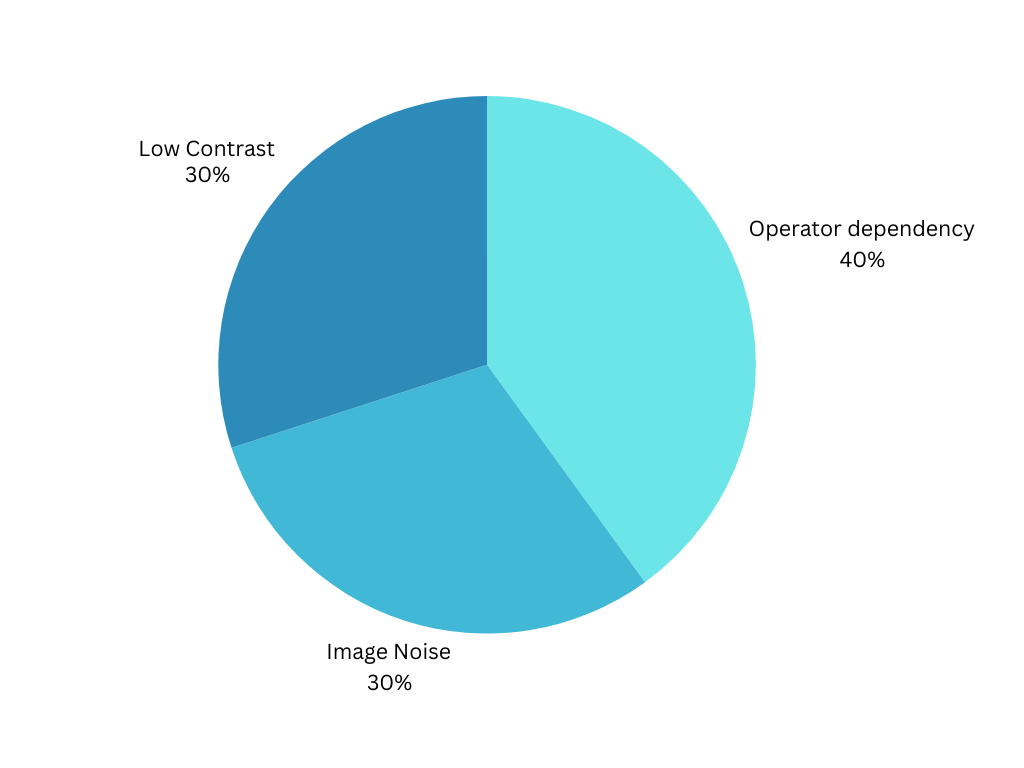
\includegraphics[width=1.0\textwidth]{introdiagram[1].png}}
    \caption{Distribution Of Diagnotic Errors}
    \label{fig:ultrasound}
\end{figure}
\vspace{10pt}
\newpage
\vspace{10pt}
\noindent The given pie chart highlights key factors contributing to diagnostic errors in ultrasound imaging: operator dependency (40), low contrast (30), and noise (30). Traditional ultrasound heavily relies on the skill of the operator, leading to subjective interpretations, while poor contrast and image noise can obscure disease detection. Your project, integrating CNN and YOLOv11 based AI models, minimizes human error by automating detection for thyroid, breast cancer, kidney stones, and liver disorders. By enhancing image processing, segmentation, and classification, it improves diagnostic accuracy, reduces reliance on operator expertise, and ensures faster, more reliable clinical decision-making, ultimately revolutionizing ultrasound-based disease detection and patient care.

\newpage
\subsection{1.2 Relevance}
\vspace{10pt}

   \noindent The ultrasonic diagnosis of an illness is challenging even for seasoned medical professionals. Misdiagnosis may occur because the quality of the images relies on factors such as the type of ultrasound machine utilized, the patient's anatomical characteristics, and the practitioner’s expertise. For instance, minor issues like neoplasms in their initial stages or nerve injury can be missed
because the images are not distinct enough. Such a delay in identifying the condition may complicate treatment procedures and even jeopardize patient health. In many regions, especially rural or
small towns, there are not sufficient specialist doctors to scan ultrasound images efficiently. Thus,
patients have to wait weeks to see an expert, which is risky for acute conditions like breast cancer
or liver disease. It is imperative to develop an automated system that can interpret ultrasound
images of pathological conditions, providing fast and reliable results and assisting physicians in
making accurate decisions. With the help of computer programs like YOLOv11 and CNNs,
our system can screen ultrasound images for four diseases: thyroid, breast cancer, kidney stones,
and liver, without relying too much on human capabilities. If the system identifies a disease, it
creates a report and suggests further action such as which doctor to visit, dietary recommendations,
or suggested exercises. This accelerates healthcare, making it more accessible and cost-effective,
even in areas with a shortage of medical professionals.
   \vspace{5pt}

\noindent Beyond diagnosis, this system extends its functionality by offering comprehensive patient support, making it a one-stop platform for medical assistance. Once a disease is detected, the system generates a detailed report, provides personalized recommendations, and directs users to experienced doctors with verified credentials for further treatment. Additionally, it enhances patient care through dietary guidelines, exercise routines, and educational resources such as YouTube videos on disease management. The platform’s financial assistance feature, which allows patients to request or donate funds, further emphasizes its social impact. By combining medical guidance and patient empowerment, this project has the potential to revolutionize remote healthcare, making advanced diagnostics and clinical support accessible to a wider population.
   \vspace{5pt}



\newpage
\subsection{1.3 Organization of the Report}
\vspace{5pt}
\noindent This report is composed of the following sections: \\[2pt]

\noindent Chapter 1: Introduction

\noindent This chapter introduces the project by discussing the background, motivation,and objectives related to integrating ultrasound imaging with clinical decision support systems. \\[2pt]

\noindent Chapter 2: Literature Review

\noindent The literature review reviews previous research on ultrasound imaging, nerve detection, and machine learning-based diagnostic tools. It highlights the challenges in existing methods and identifies areas where improvements are needed.. \\[2pt]

\noindent Chapter 3: Problem Statement

\noindent This chapter outlines the specific challenges posed by ransomware attacks, including their increasing sophistication and the limitations of traditional cybersecurity measures. It emphasizes the need for proactive strategies that can adapt to these dynamic threats. \\[2pt]

\noindent Chapter 4: Methodology

\noindent The methodology chapter details the approaches used to integrate into ransomware defense strategies. This includes the selection of tools and techniques, such as Cuckoo Sandbox for malware analysis, Random Forest classifiers for detection, and the implementation of honeypots for deception. \\[2pt]   

\noindent Chapter 5: System Architecture

\noindent This chapter describes the architecture of the proposed ransomware defense system, illustrating how various components interact. It outlines the integration of dynamic reconfiguration techniques, threat detection modules, and notification systems to create a cohesive defense mechanism. \\[2pt]

\noindent Chapter 6: Implementation

\noindent The implementation chapter discusses the practical steps taken to deploy the ransomware framework. It details the setup of the system, configuration of tools, and the challenges faced during implementation, along with solutions applied to overcome these challenges. \\[2pt]

\newpage
\noindent Chapter 7: Evaluation and Testing

\noindent This chapter evaluates the effectiveness of the implemented system through testing and analysis. It presents metrics such as detection rates, response times, and overall system performance, demonstrating the effectiveness of the attack approach against ransomware threats. \\[2pt]
	
\noindent Chapter 8: Results and Discussion

\noindent The results chapter presents the findings from the evaluation and testing phase, discussing the implications of the results. It analyzes the strengths and weaknesses of the attack approach and compares it with traditional defense mechanisms in the context of ransomware prevention. \\[2pt]

\noindent Chapter 9: Conclusion and Future Work

\noindent The Ultrasound Nerve Imaging and Clinical Decision Support System provides a reliable and accessible solution for detecting diseases like thyroid disorders, breast cancer, kidney stones, and liver conditions using ultrasound imaging . By integrating YOLOv11 for detection and CNNs for segmentation, it reduces operator dependency and improves diagnostic accuracy. In the future, the system can be enhanced by expanding disease categories, increasing dataset size for better accuracy, enabling real-time processing, and validating its clinical use through trials to further support early diagnosis and patient care. \\[2pt]
\\[2pt] 


\end{document}